%Este trabalho está licenciado sob a Licença Atribuição-CompartilhaIgual 4.0 Internacional Creative Commons. Para visualizar uma cópia desta licença, visite http://creativecommons.org/licenses/by-sa/4.0/deed.pt_BR ou mande uma carta para Creative Commons, PO Box 1866, Mountain View, CA 94042, USA.

\chapter{Vetores}\label{cap_vetor}

Neste capítulo, seguimos uma abordagem geométrica para introduzir os conceitos fundamentais e as operações básicas envolvendo vetores.

\section{Segmentos Orientados}\label{cap_vetor_sec_segorien}

O conceito de \hl{\emph{segmento orientado}} é fundamental na definição de vetores. Como o próprio nome indica, \hl{trata-se de definir uma orientação a um dado \emph{segmento de reta}}. Antes, portanto, vamos definir o que entendemos por um segmento.

\subsection{Segmento}

\hl{Sejam dados dois pontos $A$ e $B$ sobre uma reta $r$. O conjunto de todos os pontos de $r$ entre $A$ e $B$ é chamado de \emph{segmento} e denotado por $AB$.} A reta $r$ é chamada de \emph{reta suporte} e os pontos $A$ e $B$ de \emph{pontos extremos}. Consulte a Figura~\ref{cap_vetor_sec_segorien:fig:segmento}.

\begin{figure}[h]
  \centering
  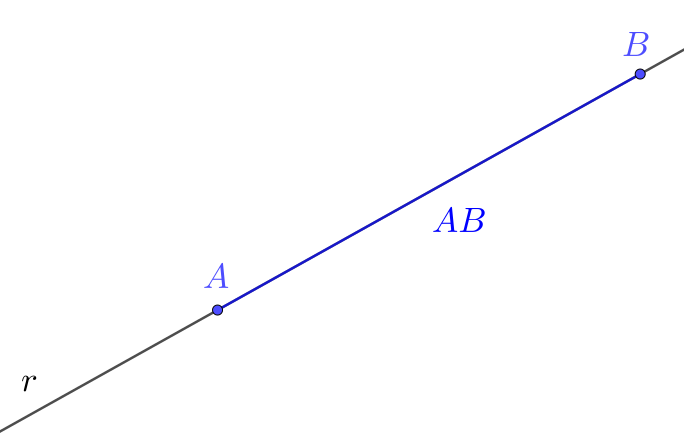
\includegraphics{./cap_vetor/dados/fig_segmento/fig.png}
  \caption{Um segmento $AB$ de uma reta (direção) $r$.}
  \label{cap_vetor_sec_segorien:fig:segmento}
\end{figure}

\subsubsection{Norma e Direção}

\hl{A \emph{norma} de um segmento $AB$ é denotada por $|AB|$ e definida como a distância entre seus pontos extremos $A$ e $B$}. Em outras palavras, é o tamanho ou comprimento do segmento\footnote{Em aplicações, a norma é medida em unidades de comprimento, metro $(m)$, no sistema internacional de unidades (SI).}. Consulte a Figura~\ref{cap_vetor_sec_segorien:fig:segmento_norma}

\begin{figure}[h]
  \centering
  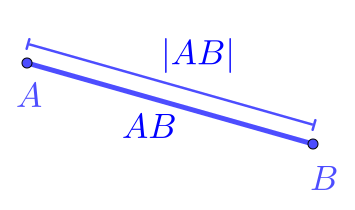
\includegraphics{./cap_vetor/dados/fig_segmento_norma/fig.png}
  \caption{Normal de um segmento $AB$.}
  \label{cap_vetor_sec_segorien:fig:segmento_norma}
\end{figure}

\hl{A \emph{direção} de um segmento $AB$ é a direção de sua reta suporte}, i.e. a direção da reta que fica determinada pelos pontos $A$ e $B$. Logo, dois segmentos $AB$ e $CD$ têm a mesma direção, quando suas retas suportes são paralelas ou coincidentes (ou seja, elas têm a mesma direção).

\begin{figure}[h]
  \centering
  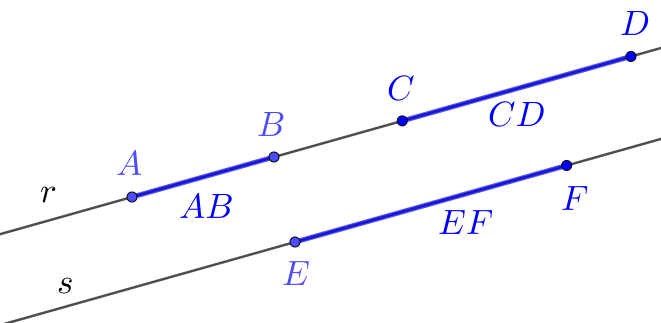
\includegraphics{./cap_vetor/dados/fig_segmento_direcao/fig.png}
  \caption{Segmentos de mesma direção $r\parallel s$.}
  \label{cap_vetor_sec_segorien:fig:segmento_direção.}
\end{figure}

\begin{ex}\label{cap_vetor_sec_segorien:ex:segmento}
  Consideramos os segmentos representados na Figura~\ref{cap_vetor_sec_segorien:fig:ex_segmento}. Observamos que $AB$ e $CD$ têm as mesmas direções, mas normas diferentes. Já, o segmento $EF$ tem a mesma norma que $AB$ (verifique!), mas tem direção diferente dos segmentos $AB$ e $CD$.
  
  \begin{figure}[h]
    \centering
    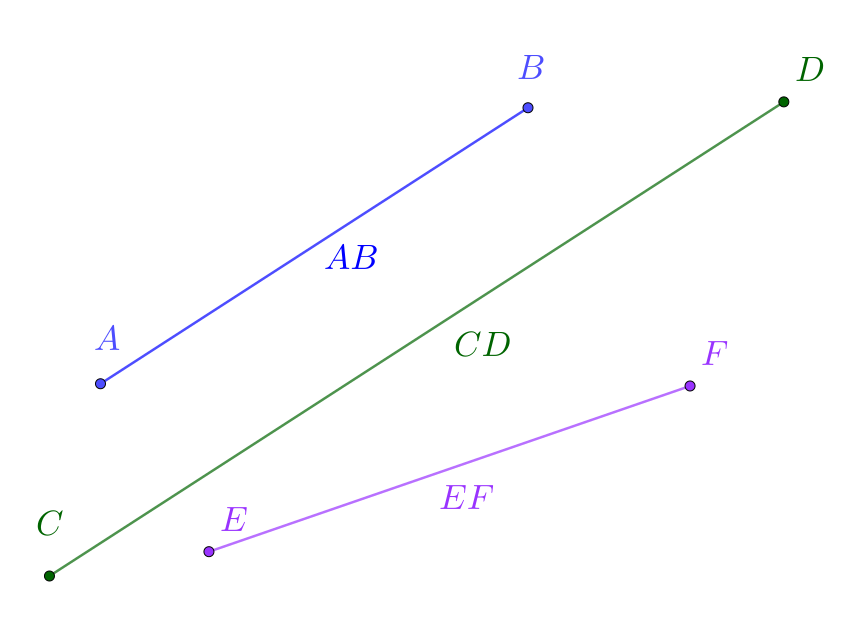
\includegraphics{./cap_vetor/dados/fig_ex_segmento/fig.png}
  \caption{Segmentos de diferentes normas e direções.}
  \label{cap_vetor_sec_segorien:fig:ex_segmento}
\end{figure}
\end{ex}

\subsubsection{Segmento Nulo}

\hl{Se $A$ e $B$ são pontos coincidentes, então chamamos $AB$ de \emph{segmento nulo} e temos $|AB| = 0$.} Observamos que a representação geométrica de um segmento nulo é um ponto, tendo em vista que seus pontos extremos são coincidentes. Como existem infinitas retas de diferentes direções que passam por um único ponto, temos que \hl{segmentos nulos não têm direção definida}.

\subsection{Segmento Orientado}

% \begin{flushright}
%   [YouTube] | \href{https://archive.org/details/definicao-segmento-orientado}{[Vídeo]} | [Áudio] | \href{https://phkonzen.github.io/notas/contato.html}{[Contatar]}
% \end{flushright}

Observamos que um dado segmento $AB$ é igual ao segmento $BA$. Agora, podemos associar a noção de \emph{sentido} a um segmento, escolhendo um dos pontos como sua \emph{origem} (ou \emph{ponto de partida}) e o outro como sua \emph{extremidade} (ou \emph{ponto de chegada}). Ao fazermos isso, definimos um \emph{segmento orientado}.

Mais precisamente, \hl{um segmento orientado $\overrightarrow{AB}$ é o segmento definido pelos pontos $A$ e $B$, sendo $A$ o ponto de partida (origem) e $B$ o ponto de chegada (extremidade)}. Consulte a Figura \ref{cap_vetor_sec_segorien:fig:seg_orientado}.

\begin{figure}[h]
  \centering
  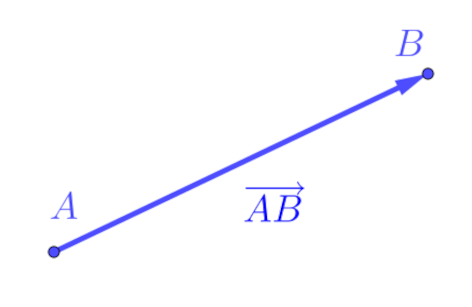
\includegraphics{./cap_vetor/dados/fig_seg_orientado/fig.png}
  \caption{Um segmento orientado $\protect\overrightarrow{AB}$.}
  \label{cap_vetor_sec_segorien:fig:seg_orientado}
\end{figure}

\subsubsection{Norma e Direção}

As noções de norma e de direção para segmentos estendem-se diretamente a segmentos orientados. Dizemos que dois \hl{segmentos orientados não nulos $\overrightarrow{AB}$ e $\overrightarrow{CD}$ têm a \textbf{mesma direção}, quando as retas $AB$ e $CD$ são paralelas ou coincidentes}. Em outras palavras, dois segmentos orientados não nulos têm a mesma direção quando suas retas suporte são paralelas ou coincidentes.

  \hl{A \emph{norma} de um segmento orientado $\overrightarrow{AB}$ é a norma do segmento $AB$}, i.e. $\left|\overrightarrow{AB}\right| = |AB|$. O segmento orientado nulo $\overrightarrow{AA}$ tem norma $\left|\overrightarrow{AA}\right|=0$ e não tem direção definida.

% \begin{ex}\label{cap_vetor_sec_segorien:ex:segorien_direcao}
%   Consideramos os segmentos orientados representados na Figura~\ref{cap_vetor_sec_segorien:fig:ex_segorien_direcao}. Os segmentos orientados $AB$ e $CD$ têm a mesma direção. Já o segmento orientado $EF$ tem direção diferente dos segmentos $AB$ e $CD$.
  
%   \begin{figure}[H]
%     \centering
%     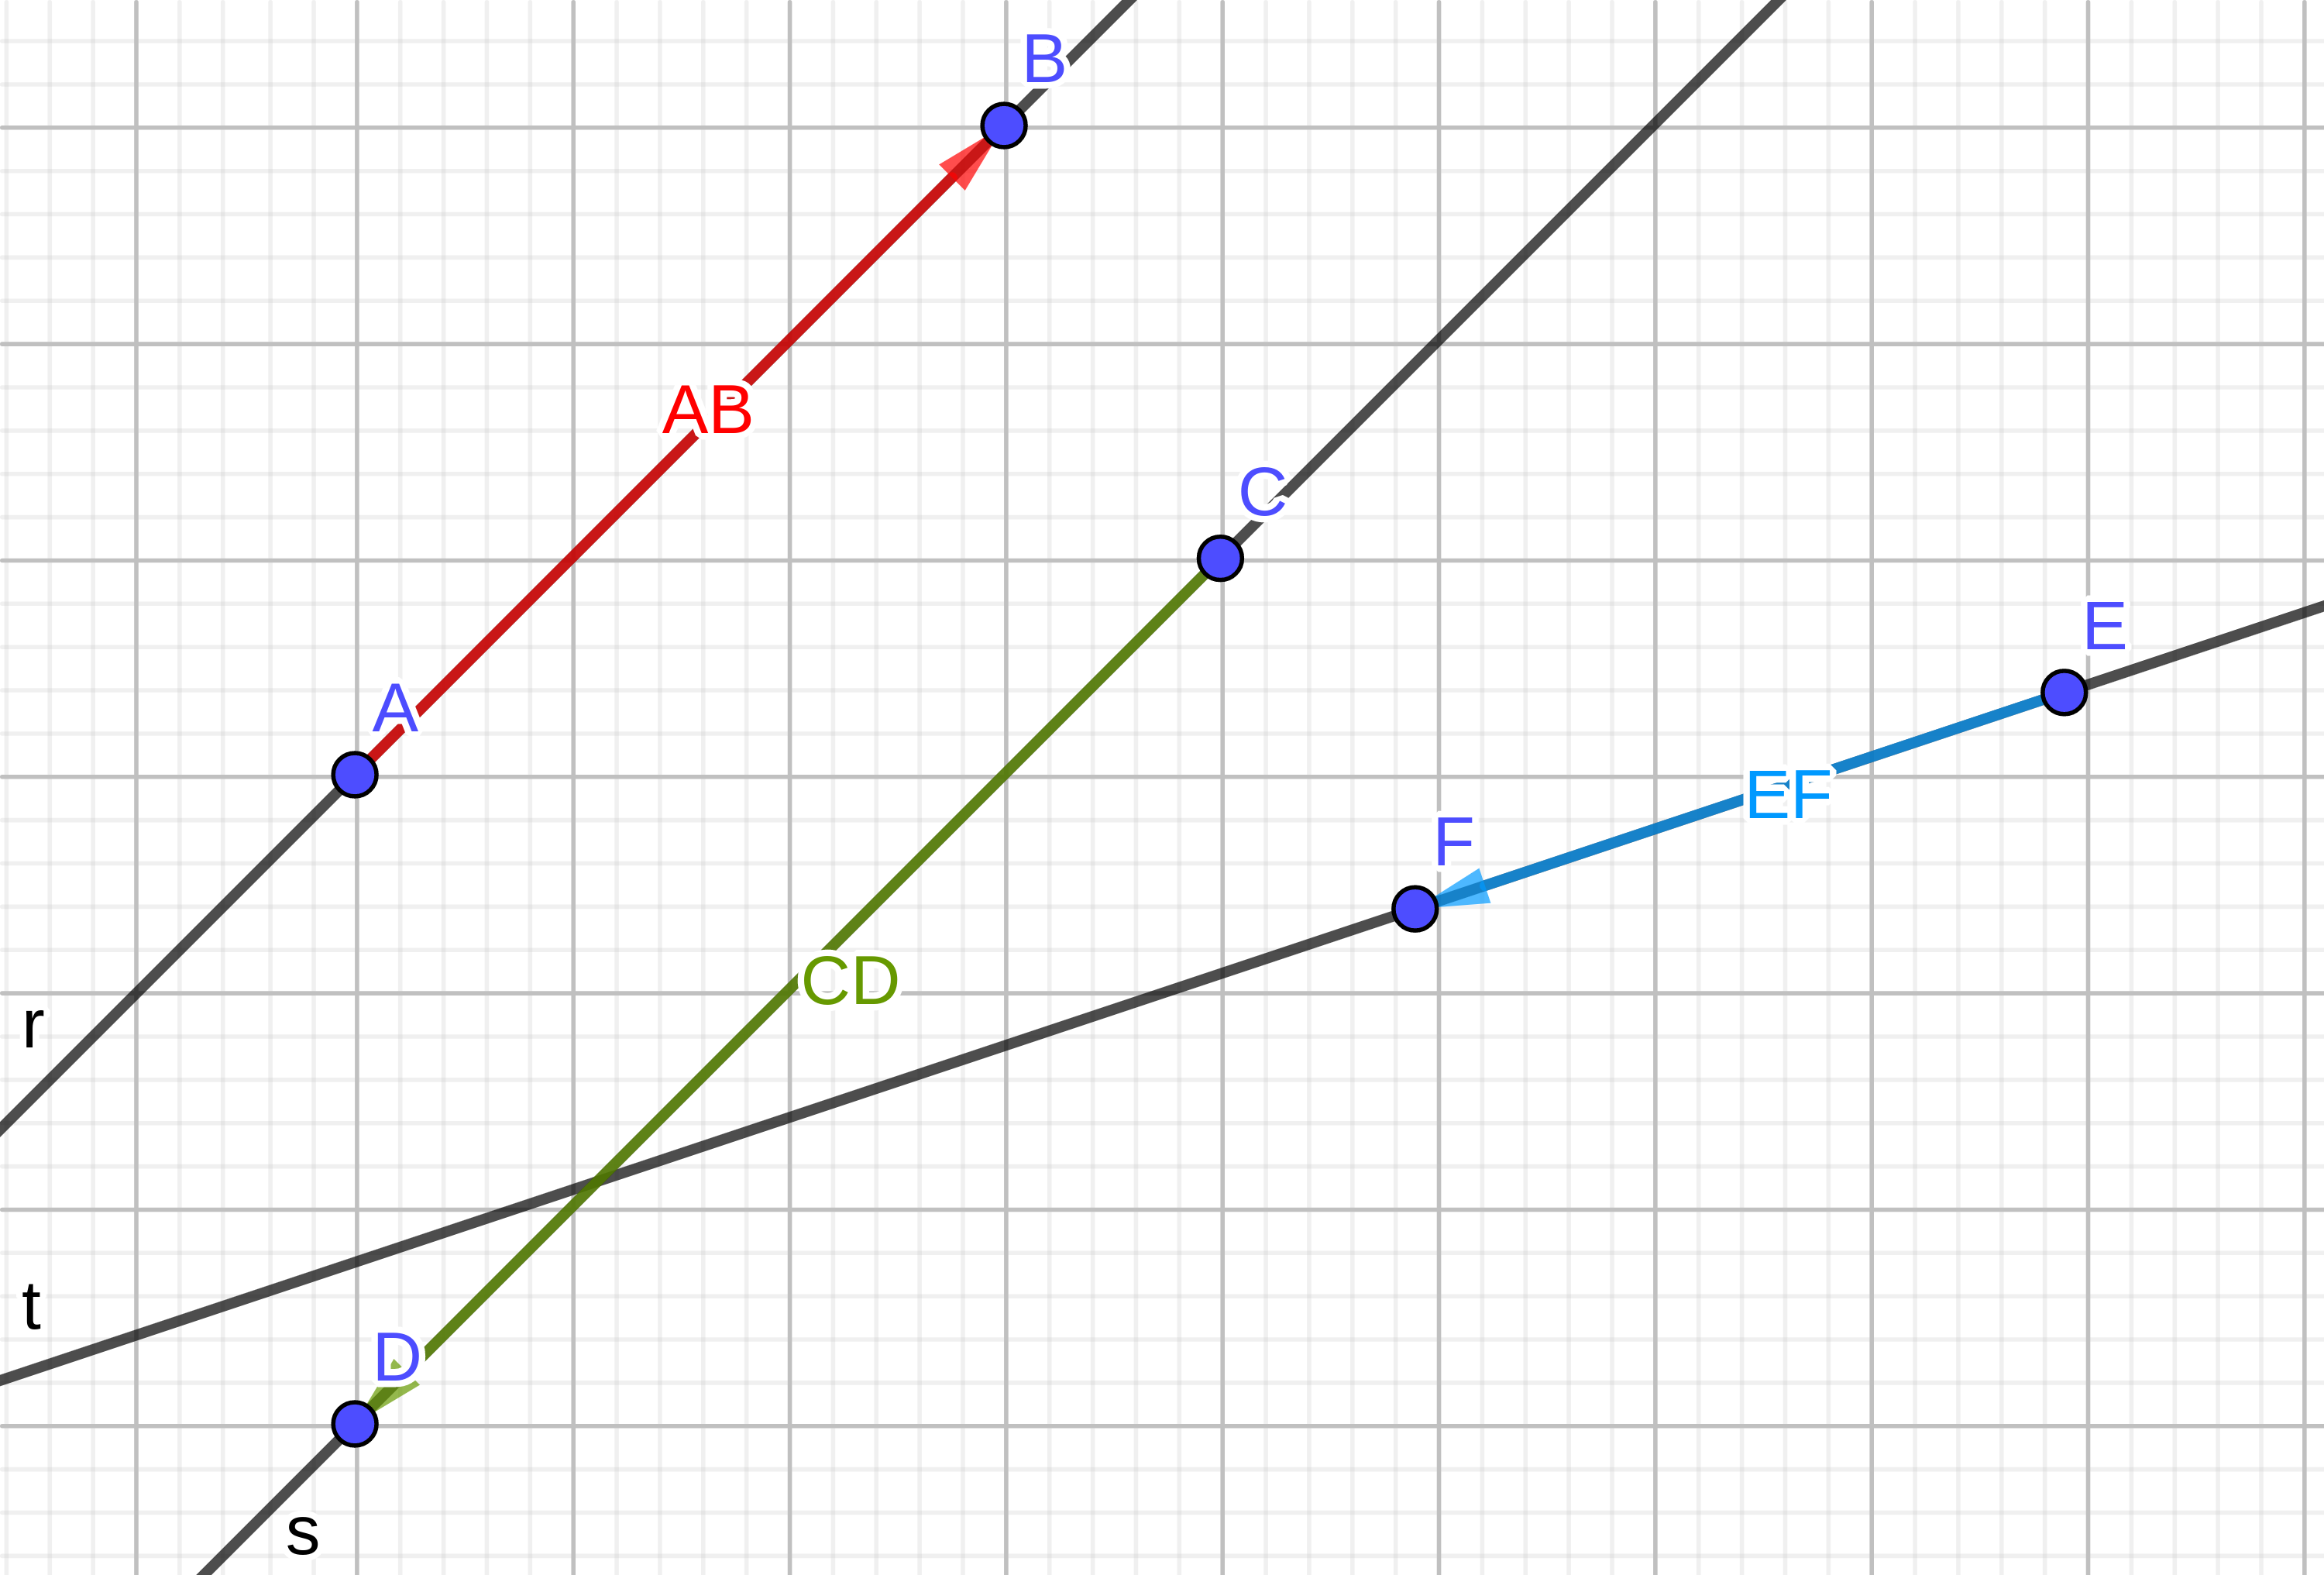
\includegraphics[width=0.7\textwidth]{./cap_vetor/dados/fig_ex_segorien_direcao/fig_ex_segorien_direcao}
%   \caption{Esboço referente ao Exemplo \ref{ex:segorien_direcao}.}
%   \label{cap_vetor_sec_segorien:fig:ex_segorien_direcao}
% \end{figure}  
% \end{ex}

\subsubsection{Comparação do Sentido}

% \begin{flushright}
%   \href{https://archive.org/details/comparacao-sentido-segmentos-orientados}{$\blacktriangleright$ Vídeo disponível!}
% \end{flushright}

\hl{Segmentos orientados $\overrightarrow{AB}$ e $\overrightarrow{CD}$ de mesma direção} podem ter o mesmo sentido ou sentidos opostos. No caso de suas retas suporte não serem coincidentes, os segmentos orientados $\overrightarrow{AB}$ e $\overrightarrow{CD}$ \hl{têm o mesmo sentido, quando os segmentos $AC$ e $BD$ não se interceptam. No contrário, caso estes se interceptam, os segmentos orientados $\overrightarrow{AB}$ e $\overrightarrow{CD}$ têm sentidos opostos}. 

\begin{ex}
  Na Figura~\ref{cap_vetor_sec_segorien:fig:segorien_sentido}, temos que os segmentos $\overrightarrow{AB}$ e $\overrightarrow{CD}$ têm o mesmo sentido. De fato, observamos que eles têm a mesma direção e que os segmentos $AC$ e $BD$ têm interseção vazia.

\begin{figure}[h]
  \centering
  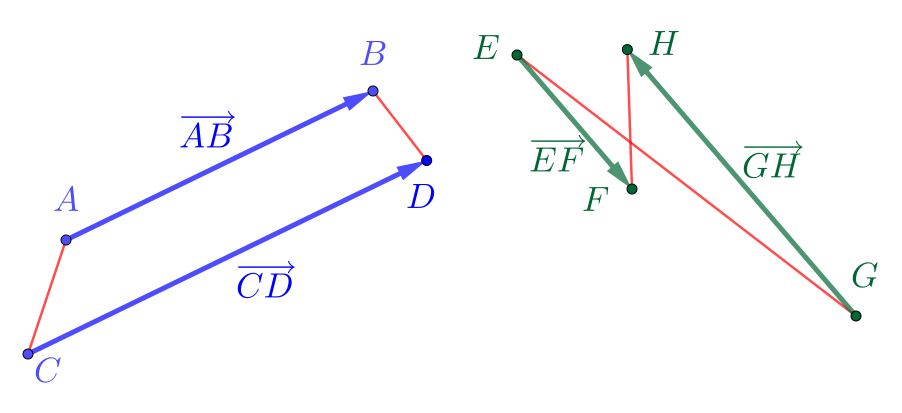
\includegraphics{./cap_vetor/dados/fig_segorien_sentido/fig.png}
  \caption{Segmentos orientados $\protect\overrightarrow{AB}$ e $\protect\overrightarrow{CD}$ de mesmo sentido. Segmentos orientados $\protect\overrightarrow{EF}$ e $\protect\overrightarrow{GH}$ de sentidos opostos.}
  \label{cap_vetor_sec_segorien:fig:segorien_sentido}
\end{figure}

Na mesma Figura~\ref{cap_vetor_sec_segorien:fig:segorien_sentido}, temos que os segmentos orientados $\overrightarrow{EF}$ e $\overrightarrow{GH}$ têm sentidos opostos, pois têm a mesma direção e os segmentos $EG$ e $FH$ se interceptam. 
\end{ex}

\begin{obs}\normalfont{(\hl{Transitividade do sentido}.)}\label{cap_vetor_sec_segorien:obs:segorin_sentido_trans}
  \hl{A propriedade de segmentos orientados terem o mesmo sentido é transitiva}. Ou seja, se $\overrightarrow{AB}$ e $\overrightarrow{CD}$ têm o mesmo sentido e $\overrightarrow{CD}$ e $\overrightarrow{EF}$ têm o mesmo sentido, então $\overrightarrow{AB}$ e $\overrightarrow{EF}$ têm o mesmo sentido.
\end{obs}

Com base na Observação~\ref{cap_vetor_sec_segorien:obs:segorin_sentido_trans}, analisamos o sentido de dois segmentos orientados e colineares escolhendo um deles e construindo um segmento orientado de mesmo sentido e não colinear. Então, analisamos o sentido dos segmentos orientados originais com respeito ao introduzido.

\subsubsection{Equipolência}

% \begin{flushright}
%   \href{https://archive.org/details/segmentos-orientados-equipolentes}{$\blacktriangleright$ Vídeo disponível!}
% \end{flushright}

\hl{Um segmento orientado não nulo $\overrightarrow{AB}$ é \emph{equipolente} a um segmento orientado $\overrightarrow{CD}$, quando $\overrightarrow{AB}$ tem a \emph{mesma norma}, a \emph{mesma direção} e o \emph{mesmo sentido} de $\overrightarrow{CD}$} (consulte a Figura~\ref{cap_vetor_sec_segorien:fig:segequipolentes}). Segmentos nulos também são considerados equipolentes entre si. 

Usamos a notação \hl{$\overrightarrow{AB} \sim \overrightarrow{CD}$} para indicar que $\overrightarrow{AB}$ é equipolente a $\overrightarrow{CD}$. Caso contrário, escrevemos \hl{$\overrightarrow{AB} \not\sim \overrightarrow{CD}$}.

\begin{figure}[h]
  \centering
  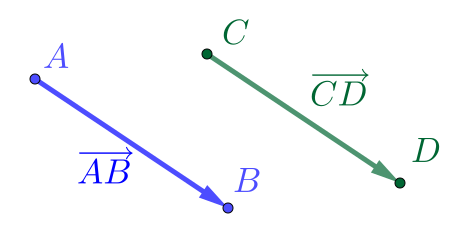
\includegraphics{./cap_vetor/dados/fig_segequipolentes/fig.png}
  \caption{Dois segmentos orientados equipolentes.}
  \label{cap_vetor_sec_segorien:fig:segequipolentes}
\end{figure}

\hl{A relação de equipolência é uma \emph{relação de equivalência}}. De fato, temos:
\begin{itemize}
\item \emph{relação reflexiva}: $\overrightarrow{AB} \sim \overrightarrow{AB}$;
\item \emph{relação simétrica}: $\overrightarrow{AB} \sim \overrightarrow{CD} \Rightarrow \overrightarrow{CD} \sim \overrightarrow{AB}$;
\item \emph{relação transitiva}: $\overrightarrow{AB} \sim \overrightarrow{CD} ~ \text{e} ~ \overrightarrow{CD} \sim \overrightarrow{EF} \Rightarrow \overrightarrow{AB} \sim \overrightarrow{EF}$.
\end{itemize}

Com isso, \hl{dado um segmento orientado $\overrightarrow{AB}$, definimos a \emph{classe de equipolência} de $\overrightarrow{AB}$ como o conjunto de todos os seus segmentos equipolentes}. O segmento $\overrightarrow{AB}$ é um \emph{representante} desta classe, a qual é denotada por $\left[\overrightarrow{AB}\right]_{\sim}$.

\subsection{Exercícios Resolvidos}

\begin{exeresol}
  Sejam dados três pontos não colineares $A$, $B$ e $D$. Escreva a área do paralelogramo determinado pelos segmentos $AB$ e $AD$ com respeito às normas deles e ao ângulo determinado por eles.
\end{exeresol}
\begin{resol}
  Começamos desenhando um paralelogramo determinado por segmentos $AB$ e $AD$. Consulte a Figura~\ref{cap_vetor_sec_segorien:fig:exeresol_paralelogramo}.

  \begin{figure}[H]
    \centering
    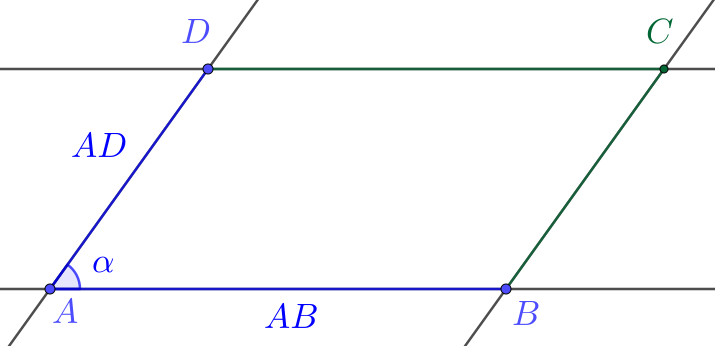
\includegraphics{./cap_vetor/dados/fig_exeresol_paralelogramo/fig.png}
    \caption{Paralelogramo determinado por segmentos $AB$ e $AD$.}
    \label{cap_vetor_sec_segorien:fig:exeresol_paralelogramo}
  \end{figure}

  Denotando por $\alpha$ o ângulo determinado pelos segmentos $AB$ e $AD$, temos que a área deste paralelogramo pode ser escrita por
  \begin{equation}
    A = |AB|\cdot |AD| \sen \alpha.
  \end{equation}
\end{resol}

\begin{exeresol}
  Mostre que $\overrightarrow{AB}\sim \overrightarrow{CD}$ se, e somente se, $\overrightarrow{BA}\sim \overrightarrow{DC}$.
\end{exeresol}
\begin{resol}
  Para mostrar que
  \begin{equation}
    \overrightarrow{AB}\sim \overrightarrow{CD} \Leftrightarrow \overrightarrow{BA}\sim \overrightarrow{DC},
  \end{equation}
  vamos primeiro mostrar a implicação, i.e. que
  \begin{equation}
    \overrightarrow{AB}\sim \overrightarrow{CD} \Rightarrow \overrightarrow{BA}\sim \overrightarrow{DC}.
  \end{equation}
  Logo, assumimos que $\overrightarrow{AB}\sim \overrightarrow{CD}$, mostramos que
  \begin{enumerate}[a)]
    \item $\left|\overrightarrow{BA}\right| = \left|\overrightarrow{DC}\right|$.
    
      De fato, temos
      \begin{equation}
        \left|\overrightarrow{BA}\right| = \left|\overrightarrow{AB}\right| \overset{\sim}{=} \left|\overrightarrow{CD}\right| = \left|\overrightarrow{DC}\right|.
      \end{equation}

    \item $\overrightarrow{BA}$ e $\overrightarrow{DC}$ têm as mesmas direções.
    
      A direção de $\overrightarrow{BA}$ é a mesma de $\overrightarrow{AB}$, pois suas retas suportes são coincidentes. Pela equipolência, essa também é a direção de $\overrightarrow{CD}$. Por fim,  $\overrightarrow{CD}$ e $\overrightarrow{DC}$ têm a mesma direção, pois suas retas suportes são coincidentes. O resultado segue por transitividade.
      
    \item $\overrightarrow{BA}$ e $\overrightarrow{DC}$ têm os mesmos sentidos.
    
      Como, por hipótese, $\overrightarrow{AB}$ tem o mesmo sentido de $\overrightarrow{CD}$, temos que os segmentos $AC$ e $BD$ não se interceptam. Isto, por sua vez, mostra que $\overrightarrow{BA}$ e $\overrightarrow{DC}$ têm o mesmo sentido.
  \end{enumerate}

  Dos items, a), b) e c), concluímos que
  \begin{equation}
    \overrightarrow{AB}\sim \overrightarrow{CD} \Rightarrow \overrightarrow{BA}\sim \overrightarrow{DC}.
  \end{equation}

  Para mostrar a recíproca, i.e. que
  \begin{equation}
    \overrightarrow{AB}\sim \overrightarrow{CD} \Leftarrow \overrightarrow{BA}\sim \overrightarrow{DC}.
  \end{equation}
  basta substituir $\overrightarrow{AB}$ ($\overrightarrow{BA}$) por $\overrightarrow{BA}$ ($\overrightarrow{AB}$) e $\overrightarrow{CD}$ ($\overrightarrow{DC}$) por $\overrightarrow{DC}$ ($\overrightarrow{CD}$) nos itens a), b) e c) demonstrados acima. Em outras palavras, a demonstração é anaĺoga. Verifique!
\end{resol}

\subsection{Exercícios}

\begin{exer}
  Complete as lacunas.
  \begin{enumerate}[a)]
    \item Seja $r$ a reta determinada pelos pontos $A$ e $B$. O segmento $AB$ é o conjunto de \underline{\phantom{pontos}} pertencentes a $r$ e que estão \underline{\phantom{entre}} $A$ e $B$ (inclusive). 
    \item A norma de um segmento $AB$ é definida como a \underline{\phantom{distância}} entre $A$ e $B$ e é denotada por \underline{\phantom{|AB|}}.
    \item Chamamos de \underline{\phantom{reta suporte}} de um dado segmento $AB$, a reta determinada pelos pontos $A$ e $B$.
    \item $AB$ é dito ser um segmento nulo, quando $A$ e $B$ são pontos \underline{\phantom{coincidentes}}.
  \end{enumerate}
\end{exer}
\begin{resp}
  a) pontos; entre; c) distância; $|AB|$; d) reta suporte; e) coincidentes;
\end{resp}

\begin{exer}
  Complete as lacunas.
  \begin{enumerate}[a)]
    \item Segmento orientado é um segmento com \underline{\phantom{sentido}} definido.
    \item Em um segmento orientado $\overrightarrow{AB}$, $A$ é chamado de \underline{\phantom{ponto de origem}} e \underline{\phantom{ponto de extremidade}}.
    \item Se as retas $AB$ e $CD$ são paralelas ou coincidentes, então $\overrightarrow{AB}$ e $\overrightarrow{CD}$ têm a mesma \underline{\phantom{direção}}.
    \item A norma de uma segmento orientado $\overrightarrow{AB}$ é definida como a norma do segmento \underline{\phantom{|AB|}}.
    \item $\overrightarrow{AB}$ e $\overrightarrow{CD}$ têm \underline{\phantom{o mesmo sentido (sentidos opostos)}} quando os segmentos $AC$ e $BD$ não se interceptam (se interceptam).
  \end{enumerate}
\end{exer}
\begin{resp}
  a) sentido; b) ponto de origem; ponto de extremidade;  c) direção; d) $|AB|$; e) o mesmo sentido (sentidos opostos); não se interceptam (se interceptam)
\end{resp}

\begin{exer}
  Complete as lacunas.
  \begin{enumerate}[a)]
    \item $\overrightarrow{AB}$ e $\overrightarrow{CD}$ são \underline{\phantom{equipolentes}} se, e somente se, $\overrightarrow{AB}$ e $\overrightarrow{CD}$ têm a mesma \underline{\phantom{direção}}, a mesma \underline{\phantom{norma}} e o mesmo \underline{\phantom{sentido}}.
    \item Pela reflexividade da relação de equipolência, $\overrightarrow{CD}\sim$ \underline{\phantom{$\overrightarrow{CD}$}}.
    \item Pela simetria da relação de equipolência, se $\overrightarrow{EF}\sim\overrightarrow{AB}$, então \underline{\phantom{$\overrightarrow{AB}\sim\overrightarrow{EF}$}}.
    \item Pela transitividade da relação de equipolência, se $\overrightarrow{CD}\sim\overrightarrow{AB}$ e \underline{\phantom{$\overrightarrow{AB}\sim\overrightarrow{EF}$}}, então $\overrightarrow{CD}\sim\overrightarrow{EF}$.
  \end{enumerate}
\end{exer}
\begin{resp}
  a) equipolentes; direção; norma; sentido; b) $\overrightarrow{CD}$; c) $\overrightarrow{AB}\sim\overrightarrow{EF}$; d) $\overrightarrow{AB}\sim\overrightarrow{EF}$
\end{resp}

\begin{exer}\label{cap_vetor_sec_segorien:fig:exer_segs_dif_normas}
  Faça o esboço de dois segmentos $AB$ e $CD$ com $|AB|\neq |CD|$ e cujas retas determinadas por eles sejam coincidentes.
\end{exer}
\begin{resp}

  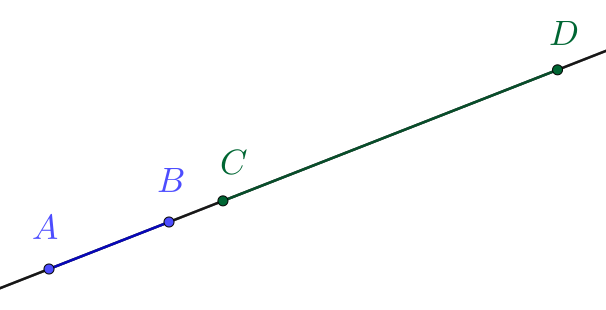
\includegraphics{./cap_vetor/dados/fig_exer_segs_dif_normas/fig.png}
\end{resp}

\begin{exer}\label{cap_vetor_sec_segorien:fig:exer_segs_nems}
  Faça o esboço de dois segmentos orientados $AB\not\sim CD$ e de mesmo sentido.
\end{exer}
\begin{resp}
  
  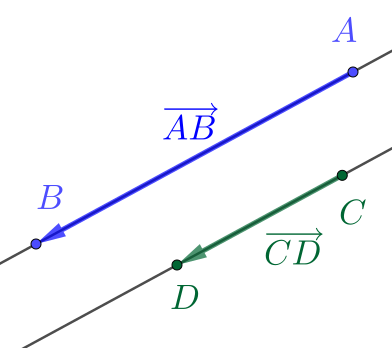
\includegraphics{./cap_vetor/dados/fig_exer_segs_nems/fig.png}
\end{resp}

\begin{exer}\label{cap_vetor_sec_segorien:fig:exer_segs_hn_s}
  Faça o esboço de dois segmentos orientados colineares, de tamanhos iguais e sentidos opostos.
\end{exer}
\begin{resp}
  
  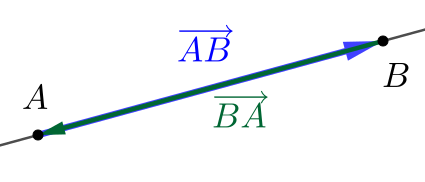
\includegraphics{./cap_vetor/dados/fig_exer_segs_hn_s/fig.png}
\end{resp}

\begin{exer}
  Mostre que $\overrightarrow{AB}\sim \overrightarrow{CD}$, então $\overrightarrow{AC}\sim \overrightarrow{BD}$.
\end{exer}
\begin{resp}
  Dica: Se $\overrightarrow{AB}$ e $\overrightarrow{CD}$ não são coincidentes, então $ABCD$ determina um paralelogramo.
\end{resp}

\begin{exer}
  Mostre que se $AC\sim CB$, então $C$ é ponto médio do segmento $AB$.
\end{exer}
\begin{resp}
  $AC\sim CB$ implica que $C\in AB$. Como $\left|\overrightarrow{AC}\right| = \left|\overrightarrow{CB}\right|$, conclui-se que $C$ é o ponto médio de $AB$.
\end{resp}

\begin{exer}
  Mostre que se $\overrightarrow{AB}$ e $\overrightarrow{CD}$ são equipolentes, então os pontos médios de $AD$ e $BC$ são coincidentes.
\end{exer}
\begin{resp}
  Dica: as diagonais de um paralelogramo interceptam-se em seus pontos médios.
\end{resp}

\ifisbook
\subsubsection{Respostas}
\shipoutAnswer
\fi

\section{Vetor}\label{cap_vetor_sec_vetor}

% \begin{flushright}
%   \href{https://archive.org/details/definicao-vetor}{$\blacktriangleright$ Vídeo disponível!}
% \end{flushright}

\hl{Um \emph{vetor} $\vec{u}$ é definido como a \emph{classe de equipolência}\footnote{Consulte a Seção~\ref{cap_vetor_sec_segorien} para a definição de classe de equipolência.} dos \emph{segmentos orientados} $\overrightarrow{AB}$ de dada \emph{norma}, dada \emph{direção} e dado \emph{sentido}}, i.e. $\vec{u} = \left[\overrightarrow{AB}\right]_{\sim}$. Qualquer $\overrightarrow{AB}\in \left[\overrightarrow{AB}\right]_{\sim}$ é uma \emph{representação do vetor} $\vec{u}$ como um segmento orientado. Consulte a Figura~\ref{cap_vetor_sec_vetor:fig:vetor}.

\begin{figure}[h]
  \centering
  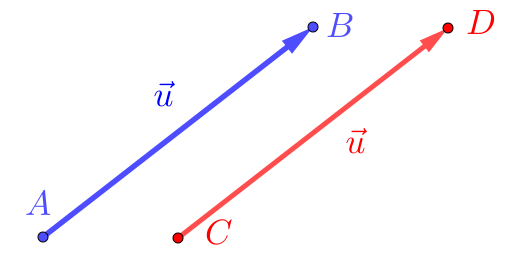
\includegraphics{./cap_vetor/dados/fig_vetor/fig.png}
  \caption{Duas representações de dado vetor $\vec{u}$.}
  \label{cap_vetor_sec_vetor:fig:vetor}
\end{figure}

\begin{obs}\normalfont{(\hl{Notação}.)}
  Para simplificar a notação, usualmente, escrevemos $\vec{u}=\overrightarrow{AB}$ no lugar de $\vec{u} = \left[\overrightarrow{AB}\right]_{\sim}$.
\end{obs}

\hl{O \emph{vetor nulo} é aquele que tem como representante um segmento orientado nulo}. É denotado por $\vec{0}$ e geometricamente representado por um ponto.

\hl{A \emph{norma} de um vetor} $\vec{u}$ é denotada por $|\vec{u}|$ e \hl{definida como a norma de qualquer uma de suas representações}. Mais precisamente, se o segmento orientado $\overrightarrow{AB}$ é uma representação de $\vec{u}$, i.e. $\vec{u} = \overrightarrow{AB}$, então
\begin{equation}
  |\vec{u}| := |\overrightarrow{AB}| := |AB|.
\end{equation}
Consulte a Figura~\ref{cap_vetor_sec_vetor:fig:vetor_norma}.

\begin{figure}[h]
  \centering
  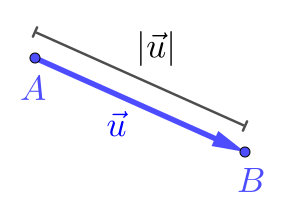
\includegraphics{./cap_vetor/dados/fig_vetor_norma/fig.png}
  \caption{Norma de um vetor $\vec{u}$.}
  \label{cap_vetor_sec_vetor:fig:vetor_norma}
\end{figure}


\begin{obs}
  $|\vec{v}| = 0$ se, e somente se, $\vec{v} = \vec{0}$.

  Seja $\vec{v} = \overrightarrow{AB}$. Lembrando que $|\overrightarrow{AB}| = |AB|$, i.e. a distância entre os pontos $A$ e $B$, segue que se $\vec{v} = \vec{0}$, então $AB$ é um segmento orientado nulo e, portanto, $0=|AB|=|\vec{v}|$. Reciprocamente, se $|\vec{v}| = 0$, então $|AB| = 0$ e, portanto, $AB$ é um segmento orientado nulo, i.e. $A$ e $B$ são pontos sobrepostos (coincidentes) e $\overrightarrow{AB} = \vec{0}$.
\end{obs}

Dois \textbf{vetores} são ditos \textbf{paralelos} quando qualquer de suas representações têm a mesma direção. De forma análoga, definem-se \textbf{vetores coplanares}, \textbf{vetores não coplanares}, \textbf{vetores ortogonais}, além de conceitos como \textbf{ângulo entre dois vetores}, etc.


\begin{ex}
  Vejamos a Figura \ref{fig:vetorrel}. Temos os vetores paralelos $\vec{u}$ e $\vec{v}$, enquanto que os vetores $\vec{s}$ e $\vec{t}$ são ortogonais (ou perpendiculares).

  \begin{figure}[H]
    \centering
    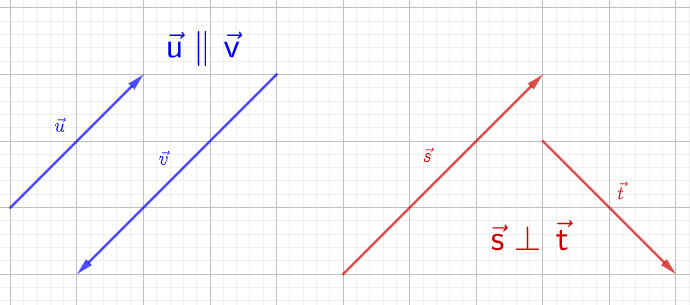
\includegraphics[width=0.7\textwidth]{./cap_vetor/dados/fig_vetorrel/fig_vetorrel.png}\\
    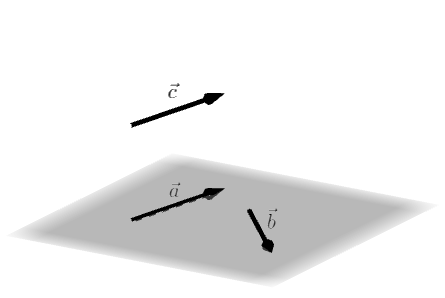
\includegraphics[width=0.5\textwidth]{./cap_vetor/dados/fig_vcolineares/fig_vcolineares.png}
    \caption{Esquerda: esboços de vetores paralelos e de vetores ortogonais. Direita: esboços de vetores coplanares.}
    \label{fig:vetorrel}
  \end{figure}
  
  Também da Figura \ref{fig:vetorrel}, temos que os vetores $\vec{a}$, $\vec{b}$ e $\vec{c}$ são coplanares. Embora, na figura $\vec{c}$ está representado fora do plano determinado pelas representações de $\vec{a}$ e $\vec{b}$, podemos tomar uma outra representação de $\vec{c}$ coplanar a estas representações.
\end{ex}


\subsection{Adição de vetores}

\begin{flushright}
  \href{https://archive.org/details/adicao-de-vetores}{$\blacktriangleright$ Vídeo disponível!}
\end{flushright}

Sejam dados dois vetores $\vec{u}$ e $\vec{v}$. Sejam, ainda, uma representação $\overrightarrow{AB}$ de $\vec{u}$ e uma representação $\overrightarrow{BC}$ do vetor $\vec{v}$. Então, define-se o vetor soma $\vec{u}+\vec{v}$ como o vetor representado por $\overrightarrow{AC}$. Veja a Figura \ref{fig:vadicao}.

\begin{figure}[H]
  \centering
  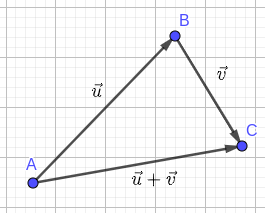
\includegraphics[width=0.5\textwidth]{./cap_vetor/dados/fig_vadicao/fig_vadicao}
  \caption{Representação geométrica da adição de dois vetores.}
  \label{fig:vadicao}
\end{figure}

\begin{obs}
  Vejamos as seguintes propriedades:
  \begin{enumerate}[a)]
  \item Elemento neutro na adição:
    \begin{equation}
      \vec{u} + \vec{0} = \vec{u}
    \end{equation}
    
    De fato, seja $\vec{u} = \overrightarrow{AB}$. Observamos que podemos representar $\vec{0} = \overrightarrow{BB}$. Logo, temos $\vec{u} + \vec{0} = \overrightarrow{AB} + \overrightarrow{BB} = \overrightarrow{AB} = \vec{u}$.

  \item Associatividade na adição:
    \begin{equation}
      (\vec{u} + \vec{v}) + \vec{w} = \vec{u} + (\vec{v} + \vec{w}).
    \end{equation}

    De fato, sejam $\vec{u} = \overrightarrow{AB}$, $\vec{v} = \overrightarrow{BC}$ e $\vec{w} = \overrightarrow{CD}$. Então, segue
    \begin{align}
      \left(\vec{u} + \vec{v}\right)+\vec{w} &= \left(\overrightarrow{AB}+\overrightarrow{BC}\right)+\overrightarrow{CD} \\
                                             &= \overrightarrow{AC} + \overrightarrow{CD} \\
                                             &= \overrightarrow{AD},
    \end{align}
    bem como,
    \begin{align}
      \vec{u} + \left(\vec{v} + \vec{w}\right) &= \overrightarrow{AB}+\left(\overrightarrow{BC}+\overrightarrow{CD}\right) \\
                                             &= \overrightarrow{AB} + \overrightarrow{BD} \\
                                             &= \overrightarrow{AD}.
    \end{align}
  \item Comutatividade da adição:
    \begin{equation}
      \vec{u} + \vec{v} = \vec{v} + \vec{u}.
    \end{equation}

    Esta propriedade pode ser demonstrada usando a regra do paralelogramo que veremos mais adiante. Veja, também, o Exercício Resolvido \ref{exeresol:vetor_comuta_adicao}.
  \end{enumerate}
\end{obs}

\subsection{Vetor oposto}

\begin{flushright}
  \href{https://archive.org/details/vetor-oposto}{$\blacktriangleright$ Vídeo disponível!}
\end{flushright}

Um \textbf{vetor} $\vec{v}$ é dito ser \textbf{oposto} a um dado vetor $\vec{u}$, quando quaisquer representações de $\vec{u}$ e $\vec{v}$ são segmentos orientados de mesmo comprimento e mesma direção, mas com sentidos opostos. Neste caso, denota-se por $-\vec{u}$ o vetor oposto a $\vec{u}$. Veja a Figura \ref{fig:voposto}.

\begin{figure}[H]
  \centering
  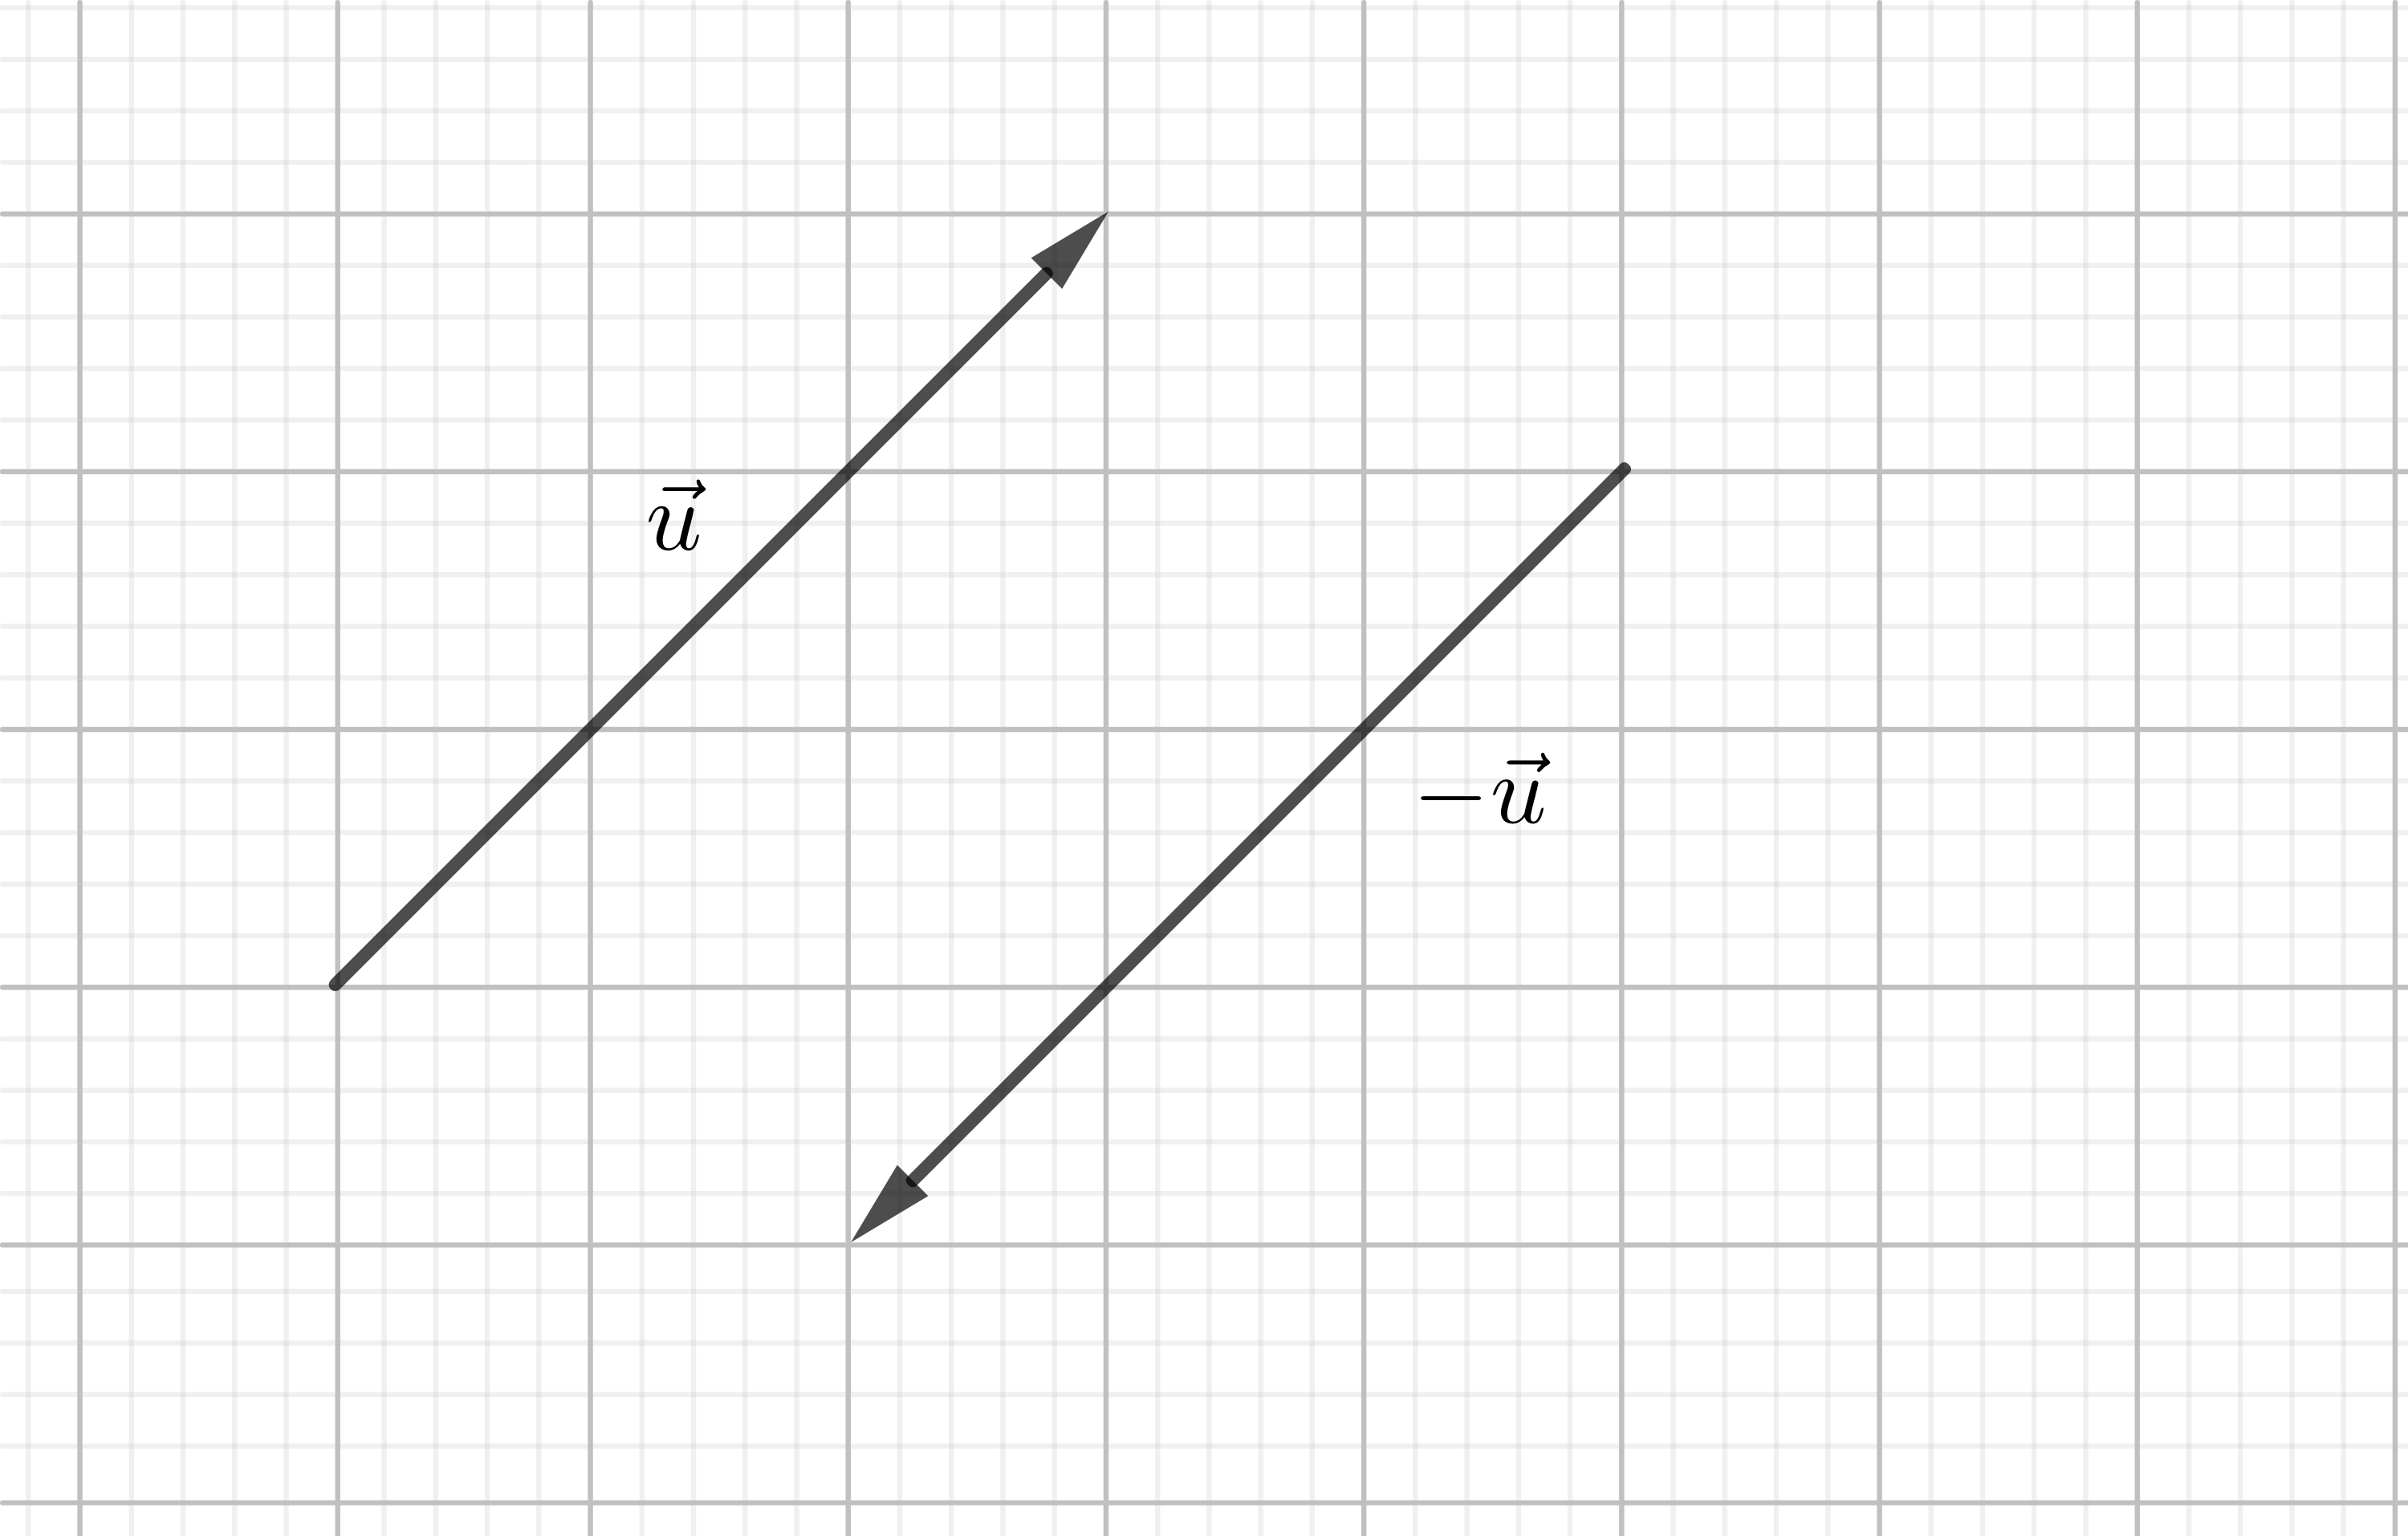
\includegraphics[width=0.5\textwidth]{./cap_vetor/dados/fig_voposto/fig_voposto}
  \caption{Representação geométrica de vetores opostos.}
  \label{fig:voposto}
\end{figure}

\begin{obs}
  $|\vec{v}| = |-\vec{v}|$.

  De fato, seja $\vec{v} = \overrightarrow{AB}$. Então, $|\vec{v}| = |AB| = |BA| = |-\vec{v}|$.
\end{obs}

\begin{obs}(Existência do oposto)
  \begin{equation}
    \vec{u} + \left(-\vec{u}\right) = \vec{0}.
  \end{equation}

  De fato, seja $\vec{u} = \overrightarrow{AB}$. Então, $-\vec{u} = -\overrightarrow{AB} = \overrightarrow{BA}$. Segue que
  \begin{align}
    \vec{u} + \left(-\vec{u}\right) &= \overrightarrow{AB} + \left(-\overrightarrow{AB}\right) \\
                                    &= \overrightarrow{AB} + \overrightarrow{BA} \\
                                    &= \overrightarrow{AA} \\
                                    &= \vec{0}.
  \end{align}
\end{obs}

\subsection{Subtração de vetores}

\begin{flushright}
  \href{https://archive.org/details/subtracao-de-vetores}{$\blacktriangleright$ Vídeo disponível!}
\end{flushright}

Sejam dados dois vetores $\vec{u}$ e $\vec{v}$. A subtração de $\vec{u}$ com $\vec{v}$ é denotada por $\vec{u}-\vec{v}$ e é definida pela adição de $\vec{u}$ com $-\vec{v}$, i.e. $\vec{u}-\vec{v}=\vec{u}+(-\vec{v})$. Veja a Figura \ref{fig:vsubtracao}.

\begin{figure}[H]
  \centering
  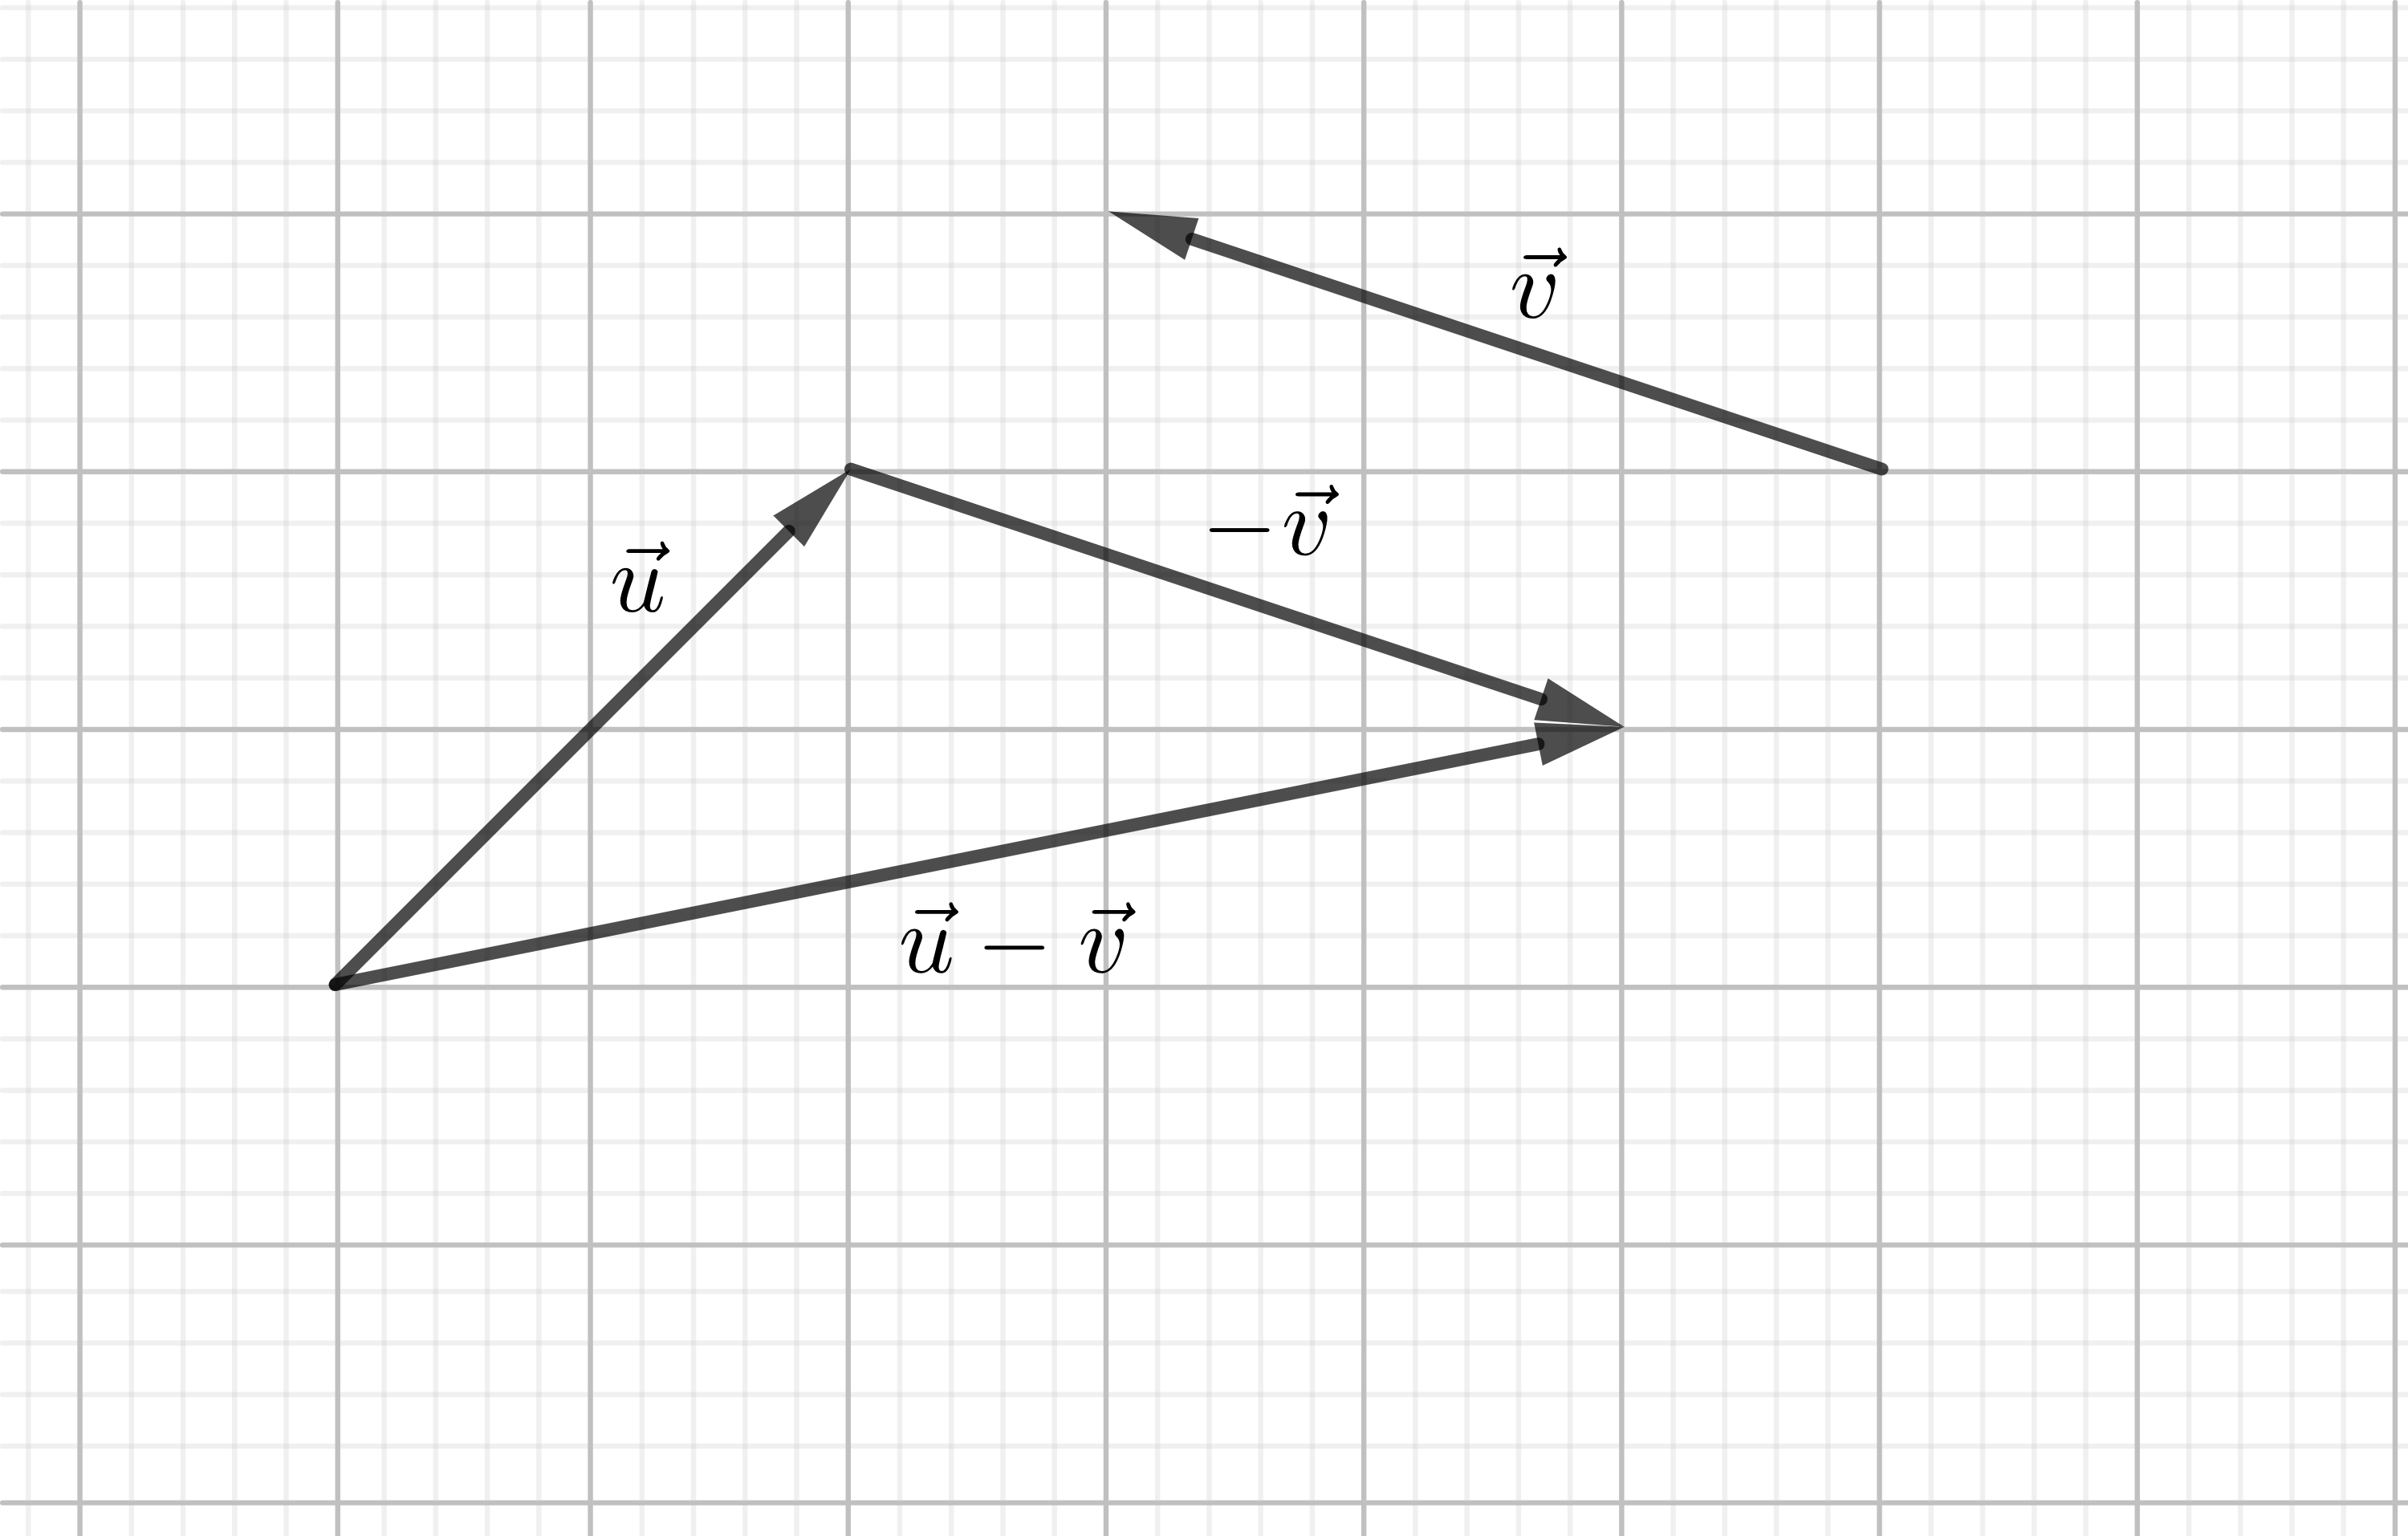
\includegraphics[width=0.5\textwidth]{./cap_vetor/dados/fig_vsubtracao/fig_vsubtracao}
  \caption{Representação geométrica da subtração de $\vec{u}$ com $\vec{v}$, i.e. $\vec{u}-\vec{v}$.}
  \label{fig:vsubtracao}
\end{figure}

\begin{obs}\normalfont{(Regra do paralelogramo)}\label{obs:vetor_regra_do_paralelogramo}
  \begin{flushright}
    \href{https://archive.org/details/regra-do-paralelogramo}{$\blacktriangleright$ Vídeo disponível!}
  \end{flushright}

  Sejam vetores não nulos $\vec{u} = \overrightarrow{AB}$ e $\vec{v} = \overrightarrow{AD}$. Seja, ainda, $C$ o vértice oposto ao $A$ no paralelogramo determinado pelos lados formados pelos segmentos $AB$ e $AD$. Então, temos $\vec{u} + \vec{v} = \overrightarrow{AC}$ e $\vec{u}-\vec{v} = \overrightarrow{DB}$. Veja a Figura \ref{fig:regrapara}.

\begin{figure}[H]
  \centering
  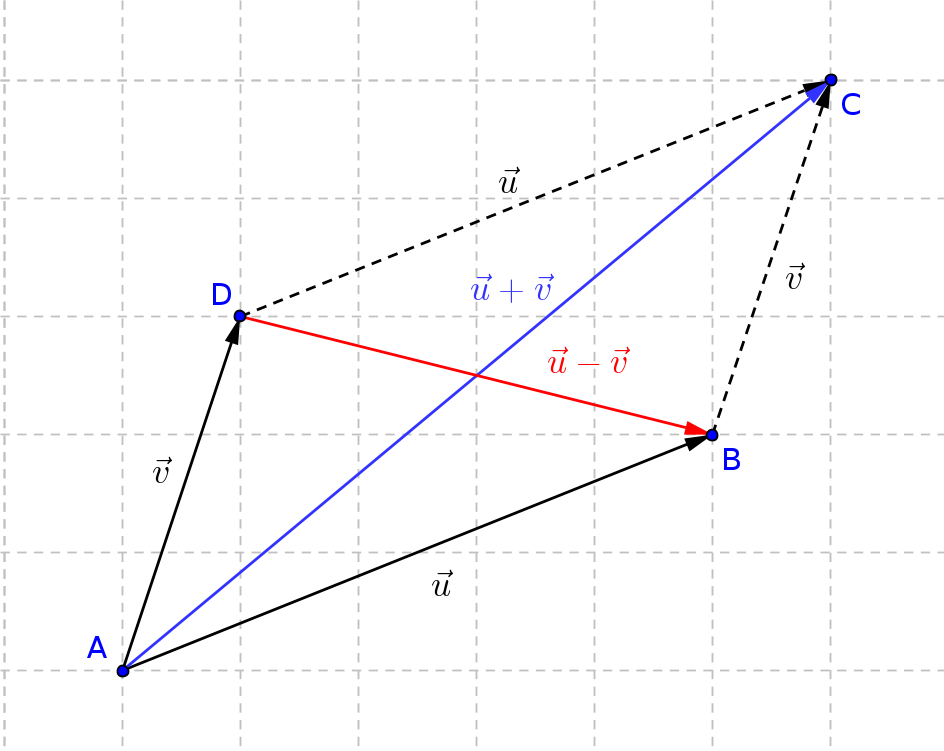
\includegraphics[width=0.6\textwidth]{./cap_vetor/dados/fig_regrapara/fig_regrapara}
  \caption{Regra do paralelogramo para a presentação geométrica da soma e da diferença de vetores.}
  \label{fig:regrapara}
\end{figure}  
\end{obs}

\subsection{Multiplicação de vetor por um escalar}

\begin{flushright}
  \href{https://archive.org/details/multiplicacao-vetor-por-escalar}{$\blacktriangleright$ Vídeo disponível!}
\end{flushright}

A multiplicação de um número real $\alpha>0$ (escalar) por um vetor $\vec{u}$ é denotado por $\alpha\vec{u}$ e é definido pelo vetor de mesma direção e mesmo sentido de $\vec{u}$ com norma $\alpha|\vec{u}|$. Quando $\alpha = 0$, define-se $\alpha\vec{u}=\vec{0}$, i.e. o vetor nulo (geometricamente, representado por qualquer ponto).

\begin{obs}
  Notamos que:
  \begin{itemize}
  \item Para $\alpha<0$, temos $\alpha\vec{u} = -(-\alpha\vec{u})$.
  \item $|\alpha\vec{u}|=|\alpha||\vec{u}|$.
\end{itemize}
\end{obs}

\begin{figure}[H]
  \centering
  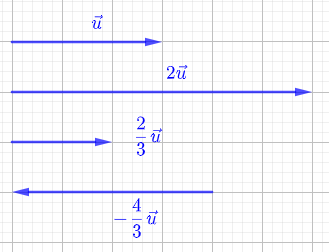
\includegraphics[width=0.6\textwidth]{./cap_vetor/dados/fig_vescalar/fig_vescalar}
  \caption{Representações geométricas de multiplicações de um vetor por diferentes escalares.}
  \label{fig:vescalar}
\end{figure}

\begin{obs}
  As seguintes propriedades são válidas:
  \begin{enumerate}[a)]
  \item Associatividade da multiplicação por escalar:
    \begin{equation}
      \alpha\left(\beta\vec{u}\right) = (\alpha\beta)\vec{u}
    \end{equation}

    De fato, em primeiro lugar, observamos que $\alpha\left(\beta\vec{u}\right)$ e $(\alpha\beta)\vec{u}$ têm a mesma direção e o mesmo sentido. Por fim, temos
    \begin{align}
      |\alpha\left(\beta\vec{u}\right)| &= |\alpha||\beta\vec{u}| \\
                                        &= |\alpha|\left(|\beta||\vec{u}|\right) \\
                                        &= \left(|\alpha||\beta|\right)|\vec{u}| \\
                                        &= |\alpha\beta||\vec{u}| \\
                                        &= |(\alpha\beta)\vec{u}|.
    \end{align}
    
  \item Distributividade:
    \begin{align}
      &(\alpha + \beta)\vec{u} = \alpha\vec{u} + \beta\vec{u}\\
      &\alpha\left(\vec{u}+\vec{v}\right) = \alpha\vec{u} + \alpha\vec{v}
    \end{align}
  \end{enumerate}
\end{obs}

\subsection{Resumo das propriedades das operações com vetores}

As operações de adição e multiplicação por escalar de vetores têm propriedades importantes. Para quaisquer vetores $\vec{u}$, $\vec{v}$ e $\vec{w}$ e quaisquer escalares $\alpha$ e $\beta$ temos:
\begin{itemize}
\item comutatividade da adição: $\vec{u}+\vec{v}=\vec{v}+\vec{u}$;
\item associatividade da adição: $(\vec{u} + \vec{v}) + \vec{w} = \vec{u} + (\vec{v} + \vec{w})$;
\item elemento neutro da adição: $\vec{u}+\vec{0}=\vec{u}$;
\item existência do oposto: $\vec{u}+(-\vec{u}) = \vec{0}$;
\item associatividade da multiplicação por escalar: $\alpha(\beta\vec{u})=(\alpha\beta)\vec{u}$;
\item distributividade da multiplicação por escalar:
  \begin{align}
    &\alpha(\vec{u}+\vec{v}) = \alpha\vec{u}+\alpha\vec{v},\\
    &(\alpha+\beta)\vec{u} = \alpha\vec{u}+\beta\vec{u};
  \end{align}
\item existência do elemento neutro da multiplicação por escalar: $1\vec{u}=\vec{u}$.
\end{itemize}

\subsection*{Exercícios resolvidos}

\begin{exeresol}
  Com base na figura abaixo, forneça o vetor $\overrightarrow{HC}$ como resultado de operações básicas envolvendo os vetores $\vec{u}$ e $\vec{v}$.
  \begin{figure}[H]
    \centering
    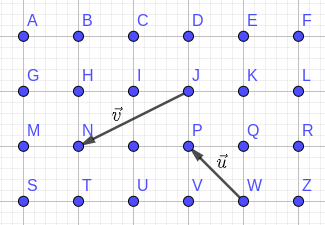
\includegraphics[width=0.7\textwidth]{./cap_vetor/dados/fig_exer_op_basicas/fig_vec_soma}
  \end{figure}
\end{exeresol}
\begin{resol}
  Vamos construir dois vetores auxiliares $\overrightarrow{HB}$ e $\overrightarrow{HI}$ a partir de operações envolvendo os vetores $\vec{u}$ e $\vec{v}$. Notamos que $\overrightarrow{HC} = \overrightarrow{HI} + \overrightarrow{HB}$.

  Começamos buscando formar o vetor $\overrightarrow{HI}$. Para tanto, observamos que $\vec{u}=\overrightarrow{NG}$ e, portanto, $\vec{v}+\vec{u}=\overrightarrow{JG}$. Com isso, obtemos que
  \begin{align}
    \overrightarrow{HI} &= -\frac{1}{3}\overrightarrow{JG} \\
                        &= -\frac{1}{3}(\vec{v}+\vec{u}).
  \end{align}

  Agora, vamos formar o vetor $\overrightarrow{HB}$. Isso pode ser feito da seguinte forma
  \begin{align}
    \overrightarrow{HB} &= \overrightarrow{WQ} \\
                        &= \vec{u} + \overrightarrow{PQ} \\
                        &= \vec{u} + \overrightarrow{HI} \\
                        &= \vec{u} -\frac{1}{3}(\vec{v}+\vec{u}) \\
                        &= \frac{2}{3}\vec{u} - \frac{1}{3}\vec{v}.
  \end{align}

  Por tudo isso, concluímos que
  \begin{align}
    \overrightarrow{HC} &= \overrightarrow{HI} + \overrightarrow{HB} \\
                        &= -\frac{1}{3}(\vec{v}+\vec{u}) \\
                        &+ \frac{2}{3}\vec{u} - \frac{1}{3}\vec{v} \\
                        &= \frac{1}{3}\vec{u} - \frac{2}{3}\vec{v}.
  \end{align}
\end{resol}

\begin{exeresol}\label{exeresol:vetor_comuta_adicao}
  Mostre que $\vec{u} + \vec{v} = \vec{v} + \vec{u}$.
\end{exeresol}
\begin{resol}
  Seja $ABCD$ o paralelogramo com $\vec{u} = \overrightarrow{AB} = \overrightarrow{DC}$ e $\vec{v} = \overrightarrow{AD} = \overrightarrow{BC}$. Logo, pela regra do paralelogramo temos
  \begin{align}
    \vec{u} + \vec{v} &= \overrightarrow{AB} + \overrightarrow{BC} \\
                      &= \overrightarrow{AC} \\
                      &= \overrightarrow{AD} + \overrightarrow{DC} \\
                      &= \vec{v} + \vec{u}.
  \end{align}
\end{resol}

\subsection*{Exercícios}

\begin{exer}
  Com base na figura abaixo, qual(is) dos vetores indicados são iguais ao vetor $\overrightarrow{AB}$.
  \begin{figure}[H]
    \centering
    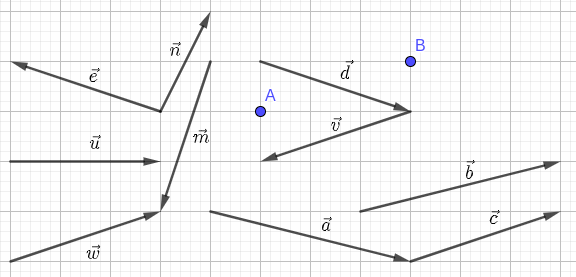
\includegraphics[width=0.7\textwidth]{./cap_vetor/dados/fig_exer_definicao_01/fig_exer_definicao_01}
  \end{figure}
\end{exer}
\begin{resp}
  $\vec{w}, \vec{c}$
\end{resp}

\begin{exer}
  Sejam $A$, $B$ e $C$ pontos dois a dois distintos. Se $\vec{b}$ é um vetor nulo, então $\vec{b}$ é igual a:
  \begin{enumerate}[a)]
  \item $\vec{0}$
  \item $\overrightarrow{AB}$
  \item $\overrightarrow{CC}$
  \item $\overrightarrow{CA}$
  \item $\overrightarrow{BB}$
  \end{enumerate}
\end{exer}
\begin{resp}
  a), c), e) 
\end{resp}

\begin{exer}
  Com base na figura abaixo, qual(is) dos vetores indicados são paralelos entre si.
  \begin{figure}[H]
    \centering
    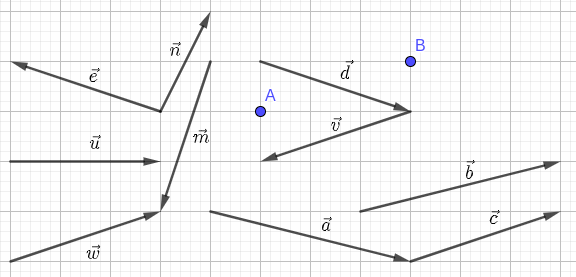
\includegraphics[width=0.7\textwidth]{./cap_vetor/dados/fig_exer_definicao_01/fig_exer_definicao_01}
  \end{figure}
\end{exer}
\begin{resp}
  $\vec{d}\parallel\vec{e}$; $\vec{c}\parallel\vec{v}\parallel\vec{w}$
\end{resp}

\begin{exer}
  Com base na figura abaixo, qual(is) dos vetores indicados são ortogonais (perpendiculares) entre si.
  \begin{figure}[H]
    \centering
    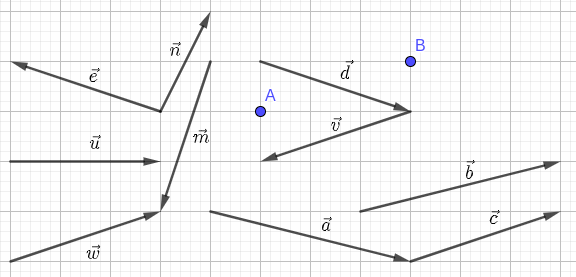
\includegraphics[width=0.7\textwidth]{./cap_vetor/dados/fig_exer_definicao_01/fig_exer_definicao_01}
  \end{figure}
\end{exer}
\begin{resp}
  $\vec{e}\perp\vec{n}$; $\vec{d}\perp\vec{n}$; $\vec{a}\perp\vec{m}$
\end{resp}

\begin{exer}
  Com base na figura abaixo, qual(is) dos seguintes são representações do vetor $\overrightarrow{v}+\overrightarrow{u}$?
  \begin{enumerate}[a)]
  \item $\overrightarrow{JG}$
  \item $\overrightarrow{QN}$
  \item $\overrightarrow{AD}$
  \item $\overrightarrow{JV}$
  \item $\overrightarrow{NN}$
  \end{enumerate}
  \begin{figure}[H]
    \centering
    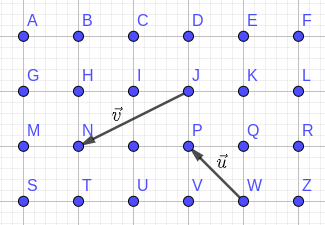
\includegraphics[width=0.7\textwidth]{./cap_vetor/dados/fig_exer_op_basicas/fig_vec_soma}
  \end{figure}
\end{exer}
\begin{resp}
  a), b)
\end{resp}

\begin{exer}
  Com base na figura abaixo, qual(is) dos seguintes são representações do vetor $\vec{w}+\vec{v}+\vec{u}$?
  \begin{enumerate}[a)]
  \item $\overrightarrow{0}$
  \item $\overrightarrow{SP}$
  \item $\overrightarrow{FP}$
  \item $\overrightarrow{v}$
  \item $\overrightarrow{AD}$
  \end{enumerate}
  \begin{figure}[H]
    \centering
    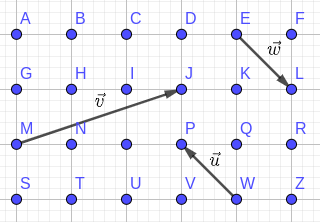
\includegraphics[width=0.7\textwidth]{./cap_vetor/dados/fig_exer_op_basicas/fig_vec_assop}
  \end{figure}
\end{exer}
\begin{resp}
  b), d)
\end{resp}

\begin{exer}
  Com base na figura abaixo, escreva os seguintes vetores como resultado de operações envolvendo $\vec{u}$ ou $\vec{v}$.
  \begin{enumerate}[a)]
  \item $\overrightarrow{QK}$
  \item $\overrightarrow{KI}$
  \item $\overrightarrow{TO}$
  \item $\overrightarrow{PE}$
  \item $\overrightarrow{FT}$
  \end{enumerate}
  \begin{figure}[H]
    \centering
    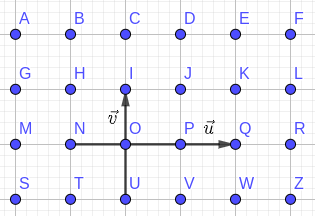
\includegraphics[width=0.7\textwidth]{./cap_vetor/dados/fig_exer_op_basicas/fig_vec_comb}
  \end{figure}
\end{exer}
\begin{resp}
  a)~$\frac{1}{2}\vec{v}$; b)~$-\frac{2}{3}\vec{u}$; c)~$\frac{1}{2}\vec{v}+\frac{1}{3}\vec{u}$; d)~$\vec{v}+\frac{1}{3}\vec{u}$; e)~$-\frac{4}{3}\vec{u}-\frac{3}{2}\vec{v}$
\end{resp}


\begin{exer}
  Seja dado um vetor $\vec{u}\neq 0$. Calcule a norma do vetor $\vec{v}=\vec{u}/|\vec{u}|$\footnote{$\vec{u}/|\vec{u}|$ é chamado de vetor $\vec{u}$ normalizado, ou a normalização do vetor $\vec{u}$.}.
\end{exer}
\begin{resp}
  $|\vec{v}|=1$.
\end{resp}

\begin{exer}
  Diga se é verdadeira ou falsa cada uma das seguintes afirmações. Justifique sua resposta.
  \begin{enumerate}
  \item $\vec{u}+\vec{u} = 2\vec{u}$
  \item $\vec{u}=-\vec{u} \Leftrightarrow \vec{u} = \vec{0}$.
  \end{enumerate}
\end{exer}
\begin{resp}
  a) verdadeira; b) verdadeira.
\end{resp}

